\documentclass[cn,blue,12pt]{elegantbook}
\input {d:/tex/preamble}

%\excludecomment{note}
%\excludecomment{solution}
%\renewcommand \tkt[1]{{\CJKunderline[hidden=true, skip=true, thickness=1pt]{#1}}}

\begin{document}

\chapter{实数基础概念}%
\label{cha:实数基础概念}

\section{知识要点}%

\begin{zsyd}
\item 实数的分类:\tkt{\(\begin{cases}
            \text{有理数}\begin{cases} \text{整数}\begin{cases} \text{自然数}\begin{cases} \text{正整数}\\ 0\end{cases}\\ \text{负整数}\\ \end{cases}\\ \text{分数}\begin{cases} \text{有限小数}\\ \text{无限循环小数}\\ \end{cases} \end{cases}\\ 
            \text{无理数}
    \end{cases}\)}
\item 无理数:\tkt{不能用两个整数的比表示}的数.也称为\tkt{无限不循环}小数,若将它写成小数形式,小数点之后的数字有\tkt{无限多个},并且\tkt{不会循环}.
    \begin{zsyd}
    \item 常见无理数类型 \tkt{\(\begin{cases} \text{开方开不尽的数:如}\sqrt{2},\sqrt{5},\textbf{注意}\sqrt{4},\sqrt[3]{-8} \text{等是有理数;}\\ \text{化简后含有根号的三角函数值,如}\sin45^\circ,\sin60^\circ,\cos30^\circ,\tan30^\circ;\\ \pi \text{及含}\pi\text{的数:如}2\pi ,\frac{\pi }{2};\\ \text{有规律但不循环的无限小数:如}0.1010010001 \cdots \text{(相邻两个1之间依次多一个0)}. \end{cases} \)}
    \item 【易错警示】 判断一个数是否为无理数, 先要\tkt{化成最简结果}, 然后再判断.如\((\sqrt{2})^2,\, 3.14\)就\tkt{不是}无理数.
    \end{zsyd}
\item 正负数的意义:正负数可以用于表示\tkt{相反意义的量}.如规定``盈(+) '' , 则``亏(-)'', ``胜(+) '' , 则``负(-)''等.
\item 数轴
    \begin{zsyd}
    \item 数轴三要素:\tkt{原点},\tkt{正方向},\tkt{单位长度}\\
            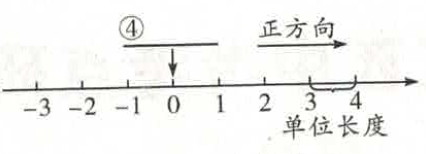
\includegraphics[width=0.8\linewidth]{wwpic/20200511012.png}
    \item \tkt{实数}与数轴上的点是一一对应的.
    \item 数轴上两点\(a,b\)的距离:\(|a-b|\),数轴上两点的中点:\(\frac{a+b}{2}\)
    \end{zsyd}
\item 相反数
    \begin{zsyd}
    \item 非零实数 \(a\) 的相反数为 \tkt{\(-a\)} ,特别地,\(0\)的相反数为\tkt{\(0\)};
    \item 实数a,b互为相反数\(\iff \) \tkt{\(a+b= 0\)} ;
    \item 互为相反数的两个数表示的点分别位于数轴上原点的\tkt{两侧}, 且到原点的距离\tkt{相等},即互为相反数的两个数在数轴上关于 \tkt{绝对值} 对称.
    \end{zsyd}
\item 绝对值
    \begin{zsyd}
    \item \(|a|=\)\( \begin{cases} a, & a>0\\ 0, & a=0\\ -a, & a<0 \end{cases} \)
    \item 绝对值具有\tkt{非负}性, 即\(|a|\)\tkt{ \(\ge \)}\(0\);
    \item 几何意义:\(|a|\)在数轴上表示\tkt{\(a\)点到原点的距离};离原点越远的数的\tkt{绝对值}越大.\(|a-b|\)表示点\(a\)到点\(b\)的\tkt{距离}.
    \end{zsyd}
\item 倒数
    \begin{zsyd}
    \item 非零实数a的倒数是 \tkt{\(\frac{1}{a}\)} .
    \item 注意:\tkt{0}没有倒数.倒数等于它本身的数是\tkt{\(-1,1\)}.
    \item 实数\(a, b\)互为倒数 \(\iff\) \tkt{\(ab=1\)}.
    \end{zsyd}

\item 科学记数法
    \begin{zsyd}
    \item 表示形式:\(a \times 10^n\). 其中\tkt{\(1\le |a| <10\)}.\(n\)是整数.
    \item \(n\)的确定
        \begin{zsyd}
        \item 当原数的绝对值\tkt{\(>10\)}时\(n\)为正整数,且等于原数的\tkt{整数位数减1}或将原数变为\(a\)时小数点向左移动的位数;
        \item 当原数的绝对值\tkt{\(<1\)}时为负整数, 它的绝对值等于原数\tkt{左起第一个非零数字前所有零的个数(含小数点前的零)}或原数变为\(a\)时小数点向右移动的位数.
        \end{zsyd}
    \item 常见计数单位的科学记数法表示:1万= \tkt{\(10^{4}\)}; 1亿= \tkt{\(1\times 10^8\)};
    \item 常见计量单位的科学记数法:1 mm = \tkt{\(1\times 10^{-3}\)} m,1 nm= \tkt{\(1\times 10^{-9}\)} m;
    \item 【易错提示】用科学记数法表示数时, 要注意已知数据是否与表示数据\tkt{单位一致}.如1351亿=\tkt{\(1.351 \times 10^{11}\)},2150万=\tkt{\(2.15\times 10^3\)}万.
    \end{zsyd}
\item 精确度:一般地, 一个近似数四舍五入到哪一位, 就说这个近似数精确到哪一位, 如\(2.15643\)精确到\(0.01\)是\tkt{\(2.16\)},精确到0.1是\tkt{\(2.2\)},精确到整数位是\tkt{\(2\)}.
\item 有效数字:在一个数中,从该数的\tkt{第一个非零数字}起,直到\tkt{末尾数字}止的数字称为有效数字,如\(0.618\)的有效数字有\tkt{三个},分别是\(6,1,8\).
\end{zsyd}
\end{document}
